\documentclass[a4paper,12pt]{article}
\usepackage{blindtext}
\usepackage[english]{babel}
\usepackage[utf8]{inputenc}
%\usepackage[OT1]{fontenc}
\usepackage{mathptmx}
\usepackage[T1]{fontenc}
\usepackage{amsfonts, amsmath, amsthm, amssymb}
\usepackage{multirow}
\usepackage{tabularx}
\usepackage{listings}
\usepackage[margin=1in, a4paper, total={6in, 10in}]{geometry}
\usepackage{setspace}
%\onehalfspacing
\linespread{1.5}
\setlength{\parindent}{0pt}
\usepackage{framed}
\usepackage[dvipsnames]{xcolor}
\usepackage[most]{tcolorbox}
\usepackage{float} 
\usepackage{chngcntr}
\counterwithin*{section}{part}
\usepackage{graphicx}
\usepackage{subcaption}
\setcounter{tocdepth}{4}
\graphicspath{{/Users/mariachiaralischi/Desktop/Studio/LUISS/3 YEAR - BI/1 semester/Introduction to Quantitative Finance/Midterm project/images}}

\usepackage{hyperref}
\hypersetup{
    colorlinks = true,
    linkcolor = black,
    filecolor = black,      
    urlcolor = black,
    }

\urlstyle{same}

\colorlet{shadecolor}{orange!15}

\title{Data Analysis for Business}
\author{Maria Chiara Lischi}
\date{February - June 2023}

\begin{document}
\pagenumbering{gobble}
\begin{titlepage}
    \begin{center}
        \vspace*{1cm}
        \Huge
        \textbf {Group Assignment}\\
        \vspace{10cm}
        \LARGE
        Hand-in date:\\22.10.2023\\
        \vspace{0.5cm}
        Campus:\\BI Oslo\\
        \vspace{0.5cm}
        Examination code and name:\\\textbf{ELE 3911} Introduction to Quantitative Finance\\
        \vspace{0.8cm}
    \end{center}
\end{titlepage}

\newgeometry{left=5cm, right=2cm, top=2cm, bottom=2cm}
\pagebreak
\tableofcontents
\pagebreak
\textbf{\Large Summary}\\
\hfill \break
This paper serves as a comprehensive response to the coursework assignment for the course Introduction to Quantitative Finance. The assignment primarily involves the analysis of a specific dataset: P2Ploans, which has been examined and processed using the R programming language. For the reader's convenience, the complete R code, accompanied by detailed explanatory comments written in Markdown, has been included as an appendix to this paper. The various code sections are systematically enumerated to simplify reference whenever they are cited in this text. This solution paper addresses the assignment's questions by furnishing precise answers and theoretical explanations where relevant.\\
\hfill \break
The dataset analysed in this assignment refers to a peer-to-peer lending platform, which is characterized by the fact that enables direct investment by individuals in retail loans (avoiding traditional financial intermediaries). In this environment, investors can individually select loans to invest in: this approach, while empowering investors, necessitates the evaluation of borrowers' creditworthiness in the construction of a personal loan portfolios. The absence of such approach poses potential risks in the form of losses and costs.\\
In this context, our analysis aims to gain insights into the characteristics of loans contained in the dataset. The variables included are: debt-to-income ratio, interest rates, internal credit ratings, loan maturities, annual payments, and risk-free interest rate. The goal of the analysis is to explore the lending dynamics, credit evaluation, and financial intricacies within the P2P lending environment.

\pagebreak
\pagenumbering{arabic}
\textcolor{Blue}{\section{Task 1}}
In this first task, our goal is to explore the properties of loans posted on the platform, focusing on the yearly loan payments variable (\textcolor{gray}{yearly\_payments}), which represents the yearly payment to the platform in USD for each loan, which are fixed in size over their duration. We will proceed by computing the present value of the first yearly payment of the loan with the largest yearly payment, and the present value of yearly payments to the platform over the duration of the whole loan (considering the risk-free rate of 1.72\% to discount payments).

\paragraph{\textcolor{Blue}{1.a}} From the computations made in \textcolor{gray}{code section 3}, the mean of the yearly payment variable is $4918.3780$, while the median is $4322.9400$. The fact that there is a significant difference among these two value suggests that the distribution is skewed; the fact that the mean is greater with respect to the median, suggests that the distribution is positively skewed (we expect the skewness value to be larger than 0), hence presents a tail on the right side.
\paragraph{\textcolor{Blue}{1.b}} Below, the plot of the distribution of yearly payments, obtained in \textcolor{gray}{code section 5}.
\begin{figure} [H]
    \centering
    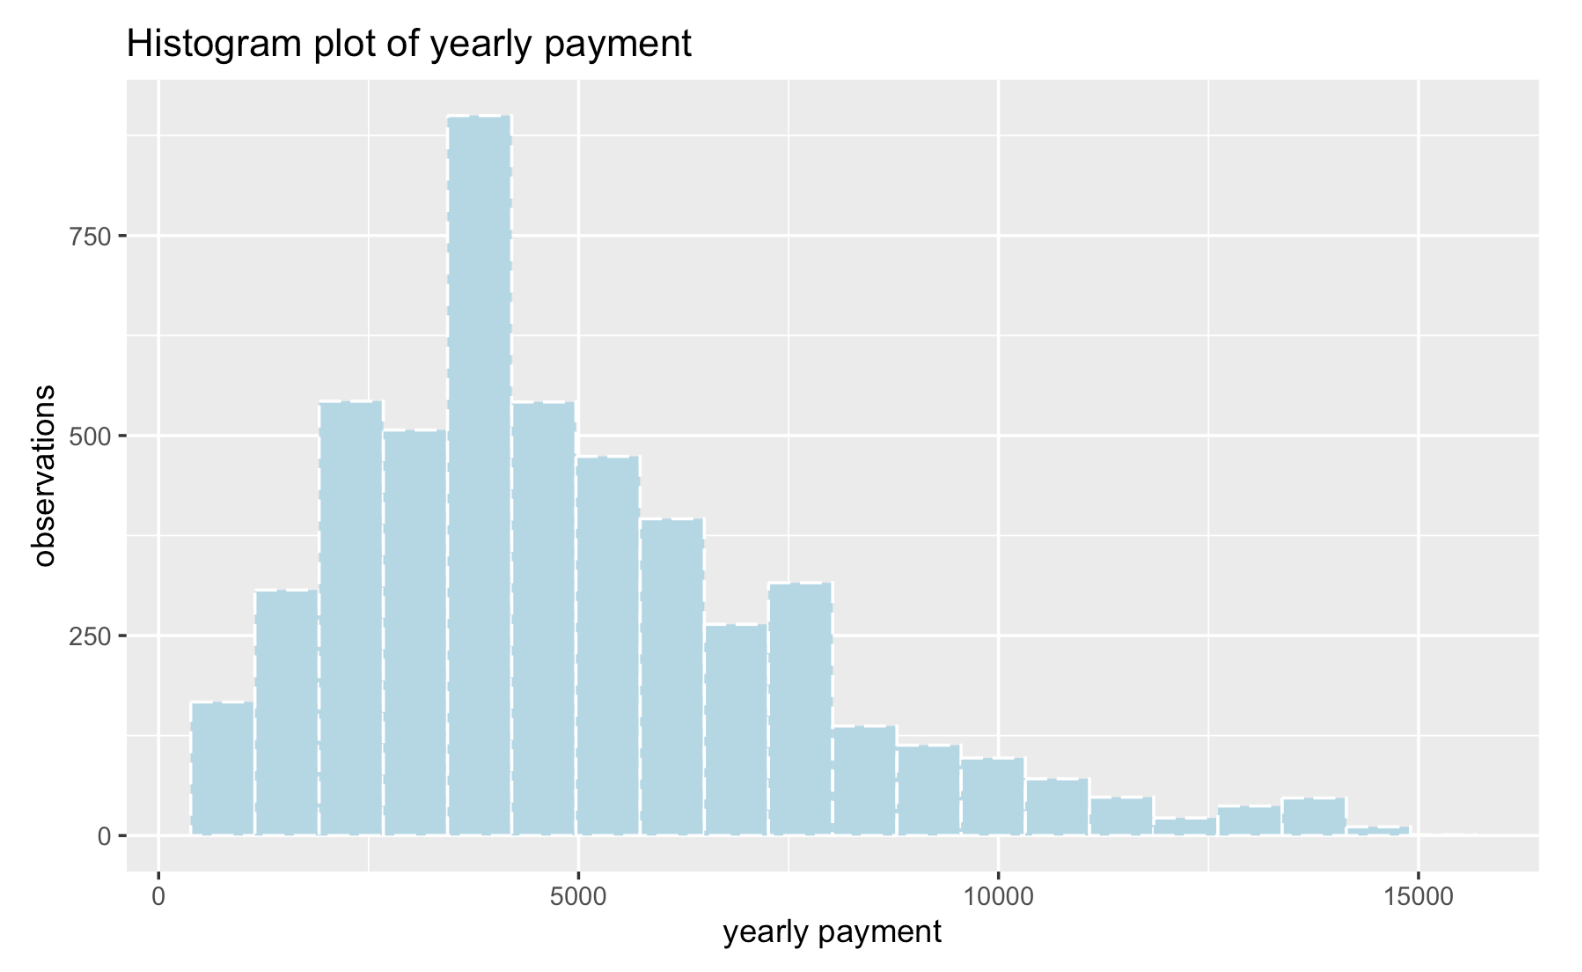
\includegraphics[width=0.9\textwidth]{plot1}
    \caption{Distribution of yearly payments} 
\end{figure}
\paragraph{\textcolor{Blue}{1.c}} The distribution of yearly payments does not appear to be symmetric: as mentioned above the fact that the the mean is greater than the median implies a right skewness. A longer tail on the right side of the distribution, indicative of a larger spread of data values on the higher end, which is not compatible with a symmetric distribution.
\paragraph{\textcolor{Blue}{1.d}} The values of skewness and kurtosis of our distribution are obtained in \textcolor{gray}{code section 6}. The skewness value of the yearly payments variable is of $1.019249$, which is in line with what we assumed in \textcolor{gray}{paragraph 1.a}. Comparing this skewness value to the one of a normal distribution, in which skewness equals zero implying symmetry, we can assert that that our distribution is not symmetric. The kurtosis value of our distribution is $4.073969$, this means that we are dealing with a leptokurtic distribution. This is not surprising because as in the histogram above we notice a high peak around the mean value. Confronting the kurtosis value with the one of a normal distribution, which is mesokurtic, with kurtosis equals 3, we assert that our distribution has a sharper peak compared to a normal. In summary, the yearly payment data is both right\-skewed and more peaked than a normal distribution.
\paragraph{\textcolor{Blue}{1.e}} Upon analysing the histogram and the computed statistics, the triangular distribution appear to be the most suitable choice to model the yearly payments variable distribution, because of its ability to capture the data's skewness and central peak. The triangular distribution is characterized by three parameters: minimum, maximum, and mode. We tuned these parameters for yearly payments data in \textcolor{gray}{code section 7}, obtaining: min = $497.7600$, max = $15020.1600$ and mode = $3900$ (the mode value was obtained by rounding the observations to the nearest hundred because the yearly payment data is continuous).
Other distributions would be worst in fitting the data: the normal would not capture the skewness as effectively, while the uniform distributions too simplistic to truly represent the distribution of yearly payments.
\paragraph{\textcolor{Blue}{1.f}} We want now to gain some insights about the loan with largest yearly payment value, whose id is $137$. Under the assumptions that payments are made at the end of each year and that the discount is at the risk-free rate of $1.72\%$, the present value of the first yearly payment made on this loan is of $14766.1800 USD$. Reference to both computations can be found in \textcolor{gray}{code section 8}. For the present value computation, the formula used is:
\begin{align}\label{present value for one year}
\Omega_{(\alpha, i)} = \Phi * \left( 1 + \frac{r_f}{100} \right)^{- i}
\end{align}
Where $\Omega$ is Present Value, $\alpha$ is the id of the loan, $i$ is the year to which the present value is calculated, $\Phi$ is Yearly Payment, and $r_f$ is risk free.\\
Substituting the specific values of loan with id $137$, we obtain:
$$\Omega_{(137, 1)} = 15020.1600 * \left(1 + \frac{1.72}{100} \right)^{- 1} = 14766.1800$$

\paragraph{\textcolor{Blue}{1.g}} The present value of yearly payments to the platform over the entire duration of the loan (considering the risk-free rate of 1.72\% for discount) is $71375.9300$. The formula used to obtain this result in \textcolor{gray}{code section 9} is:
\begin{align}\label{present value for all years}
\Omega_{\alpha} = \sum_{i = 1}^{m} \Phi * \left(1 + \frac{r_f}{100} \right)^{- i}
\end{align}
Where $\Omega$ is Present Value, $\alpha$ is the id of the loan, $m$ is the maturity of the loan, $i$ signifies each individual year included in the calculation of the present value (the formula iterates through each year of the loan's maturity, with the present value being calculated year by year), $\Phi$ is Yearly Payment, and $r_f$ is risk free.\\
Substituting the specific values of loan with id $137$, we obtain:
\footnotesize
\begin{align*}
    \Omega_{137} &= \sum_{i = 1}^{3} 15020.1600 * \left(1 + \frac{1.72}{100} \right)^{- i}\\
    &= 15020.1600 * \left(1 + \frac{1.72}{100} \right)^{- 1} + 15020.1600 * \left(1 + \frac{1.72}{100} \right)^{- 2} + 15020.1600 * \left(1 + \frac{1.72}{100} \right)^{- 3}\\
    &= 71375.9300
\end{align*}
\normalsize
\pagebreak
\textcolor{Blue}{\section{Task 2}}
In this second task, our objective is to delve into the repercussions of borrower default on the payment flows to the lending platform. The scenario we consider is one where borrowers have the option to default, resulting in a total absence of payment to the platform in all subsequent periods. We work under the assumption that loans, prior to entering default, possess a constant default probability of 0.05, irrespective of the year of payment.

\paragraph{\textcolor{Blue}{2.a}} The expected value of the first yearly payment of loan with id = 5 is of $1967.1840$. The formula used to obtain this result in \textcolor{gray}{code section 10} is:
\begin{align}\label{expected value for one year}
    \mathop{\mathbb{E}}[\Phi_{(\alpha, i)}] = p_{i} * \Phi
\end{align}
Where $\Phi$ is Yearly Payment, $\alpha$ is the id of the loan, $p_i$ signifies the probability of non-default in a specific year, denoted by $i$. It is calculated as $1$ minus the probability of default. This probability reflects the likelihood that the borrower will make the payment without defaulting in the particular year.\\
Substituting the specific values of loan with id $137$ for year $1$, we obtain:
$$\mathop{\mathbb{E}}[\Phi_{(137, 1)}] = 0.95 * 15020.1600 = 1967.1840$$
It is worth to specify that we consider the expected value of loans to equal the value of the loan multiplied for the probability of non default, plus the value obtained for the loan that has defaulted (in our case zero) multiplied by the probability of default. Computing the expected values of the payments allows to assess the likelihood of collecting each cash-flow in the future. This likelihood could be evaluated in assessing the "fair value" of the loan by taking the sum of each discounted expected cash flow.

\paragraph{\textcolor{Blue}{2.b}} Building on the same assumptions, we proceed to calculate the expected value of the final yearly payment of the loan, which is of $1775.3840$. The formula used to obtain this result in \textcolor{gray}{code section 11} is the same as (\ref{present value for all years}). However, this time the probability of non-default $p$ assumes a different value since it is computed for $i = 3$, as follows:
\begin{align*}
    p_{3} &= 1 - \underbrace{( \underbrace{pd}_{
\substack{\text{probability of} \\
  \text{default at first year}}
}
+ \underbrace{pnd * pd}_{
    \substack{\text{probability of} \\
      \text{default at second year}}
    }
    + \underbrace{pnd * pnd * pd}_{
        \substack{\text{probability of} \\
          \text{default at third year}}
        })}_{\text{probability of default by third year}}\\
        &= 1 - (0.05 + 0.95 * 0.05 + 0.95 * 0.95 * 0.05)\\
        &= 0.142625
\end{align*}
Where $pd$ is the probability of default (equal to $0.5$), and $pnd$ is the probability of non-default (equal to $1 - 0.05 = 0.95$).\\

\paragraph{\textcolor{Blue}{2.c}} The expected value of the final yearly payment of the loan is smaller with respect to the one of the first year. This is attributed to the cumulative effect of the binomial distribution. As time progresses, even if the risk remains the same for any single year, the accumulated risk over multiple years becomes more pronounced. Essentially, the cumulative effect is the stacking of individual yearly risks, leading to a compounded, larger risk over time. This means that while a borrower might not default in one particular year, the likelihood of them not defaulting over several consecutive years diminishes due to this cumulative influence.

\paragraph{\textcolor{Blue}{2.d}} To model the number of defaults in the first repayment period of payment (first year) given the probability of default we can use a binomial distribution, since we are dealing with fixed number of independent trials (5000), each with the same probability of success (probability of non default) or failure (probability of default). The parameters of the Binomial Distribution tuned for our data are:
\begin{itemize}
    \item[--] Number of trials $N$ = number of loans = $5000$
    \item[--] probability of success for each trial $p$  = probability of non default = $0.95$
    \item[--] probability of non-success for each trial $q$  = probability of default = $0.05$
\end{itemize}

\paragraph{\textcolor{Blue}{2.e}} Statistics of the distribution of the number of defaults in the first year of payments are computed in \textcolor{gray}{code section 12}. The expected number of defaults in the first year is intuitively $250$ (the value is obtained by multiplying the probability of default by the total number of loans in our dataset), the variance (given by $N * p * q$) is $237.5$, and the skewness (given by $\frac{q - p}{\sqrt{\text{variance}}}$) is $0.05839971$.

\paragraph{\textcolor{Blue}{2.f}} The sum of expected payments at the end of the first year of loans with ID values ranging from $1$ to $10$ (considering the default probability of $0.05$ for each loan and independence among them), equals $41669.5100$, as computed in \textcolor{gray}{code section 13}.

\paragraph{\textcolor{Blue}{2.g}} From a mean-variance investor perspective, it is preferable a situation in which defaults are all independent is better with respect to a situation in which defaults are perfectly correlated across borrowers. This is because when payments are independent, defaults are usually counterbalanced by other borrowers' consistent repayments, ensuring a stable cash flow (and offering investors a steadier return). From a more quantitative point of view, this can be seen in through the Markovitz Mean-Variance Portfolio Optimization Problem. The mean-variance investor, wants to pick as optimal portfolio that one characterized by the vector of weights $w$ which solves the following optimization problem:
\begin{align*}
    \max_w &\quad \lambda \mu^T w - \frac{1}{2} w^T \Sigma w\\
    \text{s.t.}&\\
    & \sum_{i=1}^m w_i = 1
\end{align*}
Noticeably, the objective function sketches the mean variance preferences of the investor, rewarding the portfolio expected returns ($\lambda \mu^T w$, where $\lambda$ a positive coefficient of preference for expected returns, while $\mu$ is the vector of expected returns of the asset involved) and penalising portfolio variability ($w^T \Sigma w$, where $\Sigma$ is the variance-covariance matrix of the assets involved) with penalty factor $0.5$. Indeed, when asset are independent, the correlation matrix is an eye matrix, and so $\Sigma$ resembles a diagonal matrix, and so the cross terms are null in the penalty part of the function. This means that the investor is only penalised for the variance of each asset, and not for the covariance between them. This is not the case when assets are perfectly correlated, where the correlation matrix is a matrix of ones, and so $\Sigma$ has positive entries everywhere. In this case, since the covariance terms are not null, the investor is penalised for the variance of each asset and for the positive covariance between assets. Thus, in the case of perfectly correlated assets, the utility function of the investor is piece-wisely lower with respect to the same utility function having independent assets, and so the optimal value of the problem defined above (i.e. the maximal utility achievable by the investor) is necessarily higher in the second case.
\pagebreak
\textcolor{Blue}{\section{Task 3}}
In this section we want to focus on the platform's system of internal ratings, which assign a risk category to each loan based on borrower and loan characteristics. The platform divides borrowers into 7 categories of internal rating: AA, A, B, C, D, E, HR.

We want to determine the extent to which interest rates, which are set in a bidding process among investors, vary with internal ratings and other observable risk characteristics.
\paragraph{\textcolor{Blue}{3.a}} We initiate our exploration by computing the mean interest rates for loans falling into the AA and HR rating groups: group AA presents a mean interest of $5.647083$, while the mean interest rate of HR group is of approximately $30.34732$. We observe that these values differs by a lot, with a difference of $24.70023$ percentage points, which is relatively is very high. 

\paragraph{\textcolor{Blue}{3.b}} The disparity in interest rates between AA and HR-rated loans can be attributed to a combination of factors, many of which are integral to the platform's risk assessment process. In detail:
\begin{itemize}
    \item [--] The borrower's debt-to-income (DTI) ratio is a pivotal factor in assessing their financial stability and influences the interest rates offered by lenders. A high DTI ratio suggests that the borrower may face challenges in meeting repayment obligations, presenting a higher default risk, hence lenders often adjust interest rates upwards.
    \item [--] The duration or term of the loan is another critical factor. Longer-term loans carry more uncertainties, arising from broader economic shifts and possible changes in the borrower's financial situation. In response to these added uncertainties, lenders typically charge higher interest rates for longer-term loans compared to shorter ones.
\end{itemize}
Also, several factors external to our dataset influence loan interest rates, such as a borrower's credit history, which provides lenders insight into their past financial behaviors, can serve as a predictor for future reliability. A tarnished history can elevate interest rates, whereas a consistent repayment record can lead to favourable rates. Additionally, the purpose of the loan can indicate its inherent risk. Loans for speculative endeavours are typically viewed as riskier than those for tangible asset acquisition. Furthermore, a borrower's employment stability plays a vital role: individuals with steady employment in well-established industries are often granted more favourable rates due to the perceived lower risk compared to those with fluctuating incomes.

\paragraph{\textcolor{Blue}{3.c}} We want now to assess the extent to which the internal ratings explain variation in the interest rate.\\
To do so, we applied a linear regression model, using the $lm()$ function in \textcolor{gray}{code section 15} of the appendix, by treating the internal ratings as a categorical variable.\\
A summary of the linear regression model obtained, is presented below:
\begin{table}[H]
    \begin{minipage}{0.5\textwidth}
        \centering
        \begin{tabular}{|c|c|}
        \hline
        \textbf{Coefficients} & \textbf{Estimate} \\
        \hline
        Intercept & 7.97951 \\
        \hline
        factor(internal rating)AA & -2.33243 \\
        \hline
        factor(internal rating)B & 3.01974 \\
        \hline
        factor(internal rating)C & 7.47501 \\
        \hline
        factor(internal rating)D & 13.42630 \\
        \hline
        factor(internal rating)E & 18.77475 \\
        \hline
        factor(internal rating)HR & 22.36781 \\
        \hline
        \end{tabular}
    \end{minipage}
    \begin{minipage}{0.5\textwidth}
        \centering
        \begin{tabular}{|c|c|}
            \hline
            \multicolumn{2}{|c|}{\textbf{Statistics}} \\
            \hline
            Multiple $R^2$ & $0.9675$ \\
            \hline
            Adjusted $R^2$ & $0.9674$ \\
            \hline
            F$-$statistic & $2.476e+04$ \\
            \hline
            p$-$value & $< 2.2e-16$ \\
            \hline
        \end{tabular}
    \end{minipage}
\end{table}
This linear regression model presents an R-squared value of $0.9675$, indicating that the considered internal ratings (AA, B, C, D, E, F) plus the intercept, explain a substantial portion of the variance in interest rates.\\
\hfill \break
By focusing our attention on the above table, it is worth noting that the built-in $lm()$ function of $R$ excluded the "$\text{factor(internal\_rating)A}$" category from the analysis. This is done to avoid the "dummy variable trap" that consists in perfect multicollinearity, where one category's values can be predicted from the values of other categories since it can be expressed as a linear combination of the others. In this context, it means that the sum of all category dummy variables for each row would be equal to the intercept value of that row. While the decision to drop one category is statistically valid (and it effectively prevents multicollinearity), it isn't the best choice when our goal is to explain variation in interest rates, because when an intercept is included in the model it introduce a bias (because it represents a baseline, which in this case, is the category A, to which all the others are compared to) making it challenging to have direct insights into the relationship between each category and interest rates.\\
To find a more accurate and interpretable representation of the interest rate variations, we built another liner regression model without an intercept term: the absence of the intercept allows a better understanding of how each category contributes to the interest rate variations, because the coefficients directly represent the expected interest rate for each rating category, rather than the difference from the omitted category (as in the previous model). This improvement can be easly visualized by analysing the following tables:
\begin{table}[H]
    \begin{minipage}{0.5\textwidth}
        \centering
        \begin{tabular}{|c|c|}
        \hline
        \textbf{Coefficients} & \textbf{Estimate} \\
        \hline
        factor(internal rating)AA & 7.97951 \\
        \hline
        factor(internal rating)AA & 5.64708 \\
        \hline
        factor(internal rating)B & 10.99925 \\
        \hline
        factor(internal rating)C & 15.45452 \\
        \hline
        factor(internal rating)D & 21.40581 \\
        \hline
        factor(internal rating)E & 26.75426 \\
        \hline
        factor(internal rating)HR & 30.34732 \\
        \hline
        \end{tabular}
    \end{minipage}
    \begin{minipage}{0.5\textwidth}
        \centering
        \begin{tabular}{|c|c|}
            \hline
            \multicolumn{2}{|c|}{\textbf{Statistics}} \\
            \hline
            Multiple $R^2$ & $0.9933$ \\
            \hline
            Adjusted $R^2$ & $0.9933$ \\
            \hline
            F$-$statistic & $1.06e+05$ \\
            \hline
            p$-$value & $< 2.2e-16$ \\
            \hline
        \end{tabular}
    \end{minipage}
\end{table}
A comparison between the $R^2$ statistic of the two model is worth attention: in the model without the intercept, its value has increased, signifying an improved explanatory power of the variation in the interest rate. Hence, this alternative approach both simplifies the interpretation of the coefficients and provides a better explanation of the variation in the interest rate.

\paragraph{\textcolor{Blue}{3.d}} Other variables included in our dataset that could explain variability in interest rates are the dti (Debt-to-Income) ratio of the borrower and the maturity of the loan. We included them as additional regressors to the previous model. The results, obtained in \textcolor{gray}{code section 17}, show that:
\begin{itemize}
    \item[--] there is a statistically significant relationship between the dti ratio and the interest rate, since the dti has a p$-$value of $5.29e-09$ (which is less than the typical significance level of $0.05$). This suggests that dti ratio has a positive effect on the interest rate, indicating that borrowers with higher debt-to-income ratios are associated with higher interest rates.
    \item[--] there is not a statistically significant relationship between the maturity and the interest rate, since the maturity has a relatively high p$-$value of $0.217$, which is not statistically significant (greater than $0.05$). Hence, the inclusion of maturity as a regressor does not substantially improve the model's explanatory power nor the regression's fit.
\end{itemize}

\paragraph{\textcolor{Blue}{3.e}} Our analysis indicate that the internal ratings already incorporate most of the information contained in the other variables in the dataset with respect to explaining variability in the interest rate.
\pagebreak
\textcolor{Blue}{\section{Task 4}}
The goal of this task is to simulate the sum of the first year of payments to the platform for rating groups E and HR, under the assumptions that each borrower either makes payment or defaults (pays \$0) with a probability given by its rating group, and that that default is independent across borrowers. 
The probability of default for each rating group is described in the table below:
\begin{table}[H]
    \centering
    \begin{tabular}{|c|c|c|c|c|c|c|c|}
        \hline
        AA & A & B & C & D & E & HR \\
        \hline
        0.01 & 0.02 & 0.03 & 0.05 & 0.08 & 0.15 & 0.30 \\
        \hline
    \end{tabular}
\end{table}
\paragraph{\textcolor{Blue}{4.a}} In \textcolor{gray}{code section 18} We executed the prescribed simulation as follows: First, we assembled a portfolio comprising loans exclusively categorized with internal ratings of "E" or "HR" from the provided dataset. Subsequently, we conducted 1000 simulations to calculate the total portfolio value, defined as the sum of payments from loans that did not default. The determination of whether each loan defaults or not was made by generating random samples from a Bernoulli distribution. These thresholds were determined by the probability of default corresponding to the internal rating groups of the loans. From the results of the 1000 portfolio simulations, we constructed the following histogram: 
\begin{figure} [H]
    \centering
    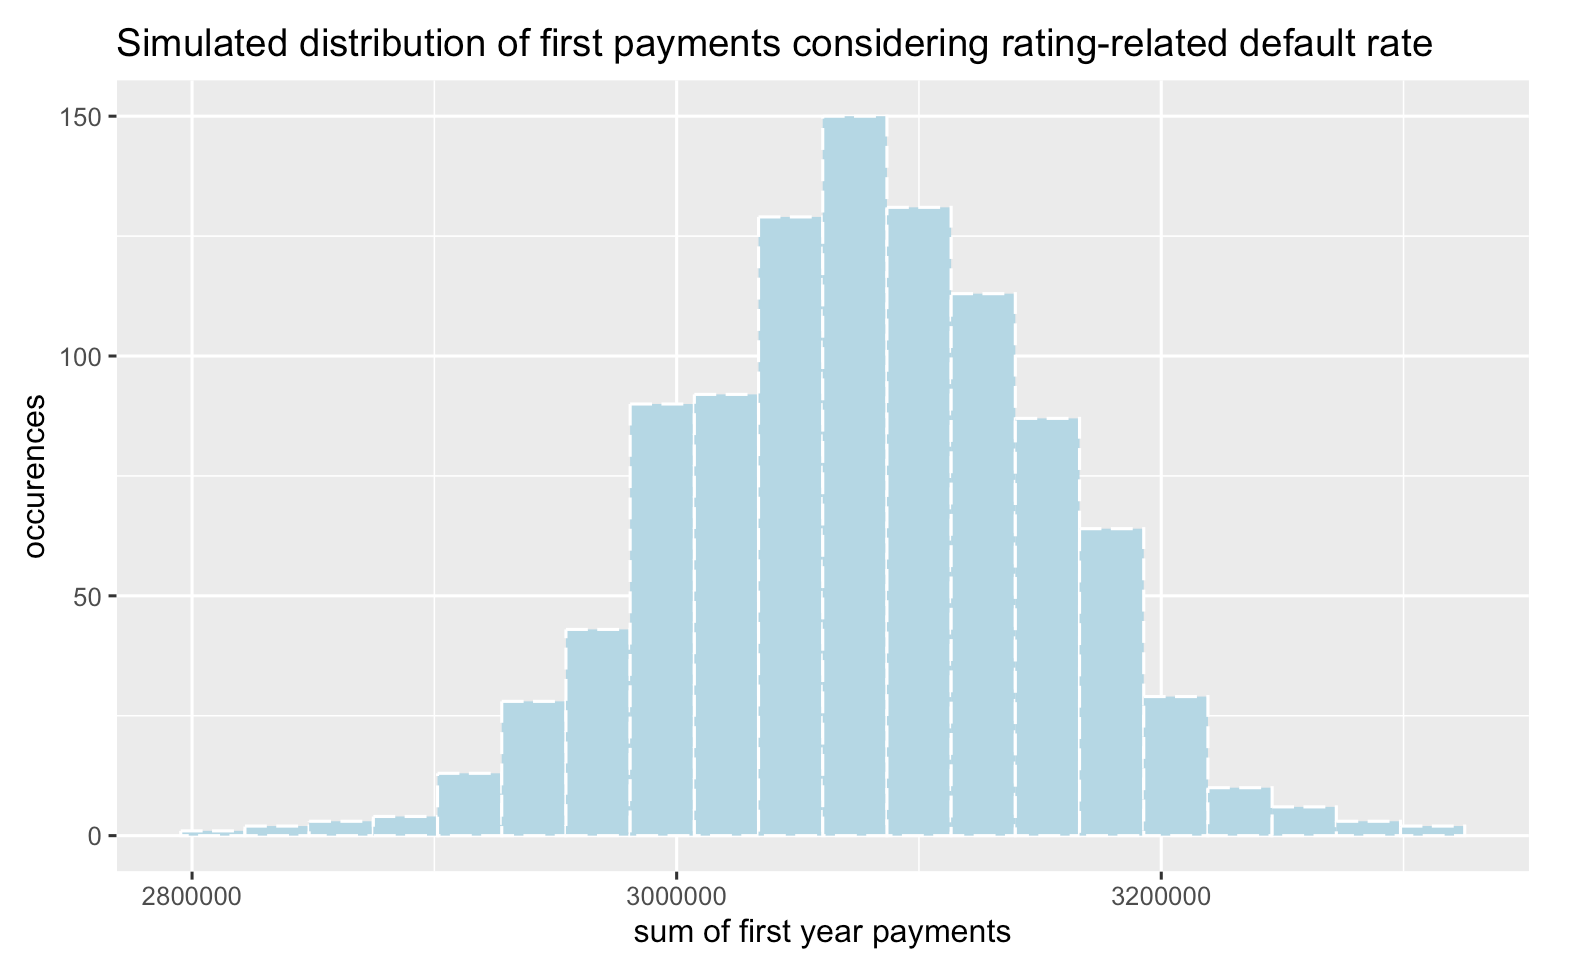
\includegraphics[width=0.9\textwidth]{plot2}
    \caption{Simulated distribution of first payments considering rating-related default rate} 
\end{figure}
\paragraph{\textcolor{Blue}{4.b}} The histogram above closely resembles a normal distribution: this can be attributed to the Central Limit Theorem (CLT), which suggests that the distribution of the sum of a large number of independent, identically distributed random variables tends to be approximately normal. In our context, as we accumulate the values of non-defaulted loans across multiple simulations, the histogram's shape converges towards a normal distribution because of the large number of samples and the independent nature of each simulation.
\paragraph{\textcolor{Blue}{4.c}} The mean of the sum of payments over the 1000 simulations is $3076123.0000$ while the standard deviation is $74304.5300$. These values are obtained in \textcolor{gray}{code section 19}.\\
We also computed the expected value of the sum of payments in \textcolor{gray}{code section 20}. Its value equals $3369243.0000$, which is in line with the mean value obtained above. This is not surprising because the expected value is a measure of the central tendency of a distribution, and it is calculated as the sum of the product of each possible value of the random variable and its probability (in our case, the sum of the product of each possible value of the sum of payments and its probability).
\paragraph{\textcolor{Blue}{4.d}} The 95\% Value at Risk (VaR) for total payments across the 1000 simulations, computed in \textcolor{gray}{code section 21} is $2956333$: this means that there is a 95\% probability that the portfolio will not lose more than $\$2956333$ over the given time period of the first year. The VaR is in fact a measure of the risk of investments: it indicates the maximum loss with a given probability and time horizon: it is calculated as the difference between the initial portfolio value and the value at the end of the time period, multiplied by the confidence level.

\end{document}